\chapter{Introdu��o}
\label{cap:introducao}
\section{Motiva��o}
\quad Em 2015 o programa AlphaGo, desenvolvido pela Alphabet Inc.'s, se tornou a primeira IA 
(intelig�ncia artificial) a ganhar de um jogador profissional de Go sem nenhum tipo de handicap.  
Feitos como este j� aconteceram antes, como por exemplo o famoso computador Deep Blue que
derrotou Garry Kasparov quando ele tinha o t�tulo de campe�o mundial. Apesar disto ter ocorrido 
em 1997, o jogo de Go era considerado por muitos o jogo mais complexo que existe e portanto, 
muito dificil de se criar uma IA.\\

\quad O resultado da AlphaGo se mostrou t�o impressionante que foi inclusive considerado um dos
maiores avan�os cient�ficos do ano e atraiu aten��o de todo o globo.  Diante disto o estudo de
"machine learning"e dos algor�tmos que permitiram tal feito se mostram de grande import�ncia,
n�o somente pelo o que j� conquistaram, mas principalmente pelas possibilidades que podem trazer.

\section{O jogo de Hex}
\quad Hex � um jogo de tabuleiro abstrato inventado pelo matem�tico dinamarqu�s Piet Hein em 1942 e
introduzido  no instituto Niels Bohr. Em 1948 outro matem�tico, John Nash, sem ter conhecimento da
inven��o de Piet re-inventou o jogo e o popularizou quando o introduziu na Universidade de Princeton.\\

\quad Hex � jogado por 2 jogadores em uma grade hexagonal que teoricamente pode ter tamanho e forma 
vari�veis. Apesar disto o tabuleiro tradicional � construido na forma de um losango com dimens�es 11x11 
ou 13x13 e cada par de lados opostos recebe uma cor distinta. Durante a partida cada jogador recebe pe�as 
de uma dessas cores e se alternam colocando-as em espa�os vazios do tabuleiro. O objetivo do jogo � criar
um caminho utilizando suas pe�as de forma a conectar os lados opostos do tabuleiro que estejam marcados
com a sua cor.


\begin{figure}[H]
  \centering
  \subfloat[Jogo em progresso]{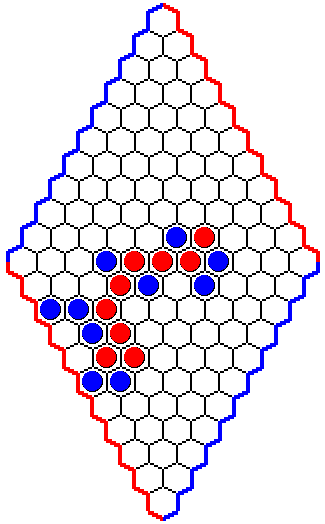
\includegraphics[angle=90, width=0.4\textwidth]{progress_hex.png}\label{progress_game}}
  \hfill
  \subfloat[Jogo finalizado]{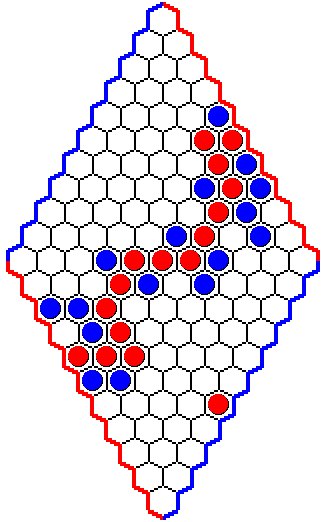
\includegraphics[angle=90, width=0.4\textwidth]{end_hex.png}\label{end_game}}
  \caption{O jogo de Hex.}
\end{figure}

\section{Estrutura do Trabalho}